\documentclass[12pt]{article}
\usepackage{comment} % enables the use of multi-line comments (\ifx \fi) 
\usepackage[english,german]{babel} 
\usepackage[utf8]{inputenc}
\usepackage{fancyhdr}
\usepackage{graphicx}
\usepackage[article, total={6in, 8in}]{geometry}
\usepackage{float}
\usepackage{wrapfig}
%\usepackage[onehalfspacing]{setspace}
\usepackage{url}
\usepackage{tabularx}
\usepackage{pdfpages}
\usepackage{wrapfig}
\usepackage[T1]{fontenc}% wichtig für Trennung von Wörtern mit Umlauten
\usepackage{microtype}% verbesserter Randausgleich
\setlength{\headheight}{21.4pt}
\usepackage{apacite}
\usepackage{eurosym}
\usepackage{amsmath}
\DeclareMathOperator{\EX}{\mathbb{E}}% expected value
\numberwithin{equation}{section}
% Special characters
\usepackage{eucal}
% math. alphabet
\usepackage{amssymb}
\usepackage{scrpage2}%
\DeclareMathOperator*{\argmax}{argmax}
\DeclareMathOperator*{\max}{argmax}

%%%% footer and header %%%%
\usepackage{scrpage2}%
\pagestyle{scrheadings}%  S
\clearscrheadfoot% 
\setheadwidth{text}%
\automark{section}% 
\ihead{\textbf{\pagemark}}
\renewcommand{\sectionmark}[1]{\markright{\ #1}} 
\ohead{\rightmark}
\setheadsepline{0.5pt}
%%%% \footer and header %%%%

\begin{document}

\begin{titlepage}
	\centering	
	{\scshape\LARGE Hochschule Bremerhaven \par}
	\vspace{1cm}
	{\scshape\Large Exposé für eine Bachelorarbeit zum Thema:\par}
	\vspace{1.5cm}
	{\huge\bfseries Reinforcement Learning\par}
	\vspace{2cm}
	{\Large\itshape Theoretische Grundlagen der tabellarischen Lernmethoden und praktische Umsetzung am Beispiel eines Ameisen-Agentenspiels
	\par}
	\vfill
	\begin{tabularx}{\textwidth}{lX}
		Autor: & Jan Löwenstrom \\
		Matrikelnr.: & 34937 \\
		Erstprüfer: & Prof. Dr.-Ing. Henrik Lipskoch \\
		Zweitprüfer: & Prof. Dr. Nadija Syrjakow \\
	\end{tabularx}  
    \vfill

% Bottom of the page with current date
	{\large \today \par}       
\end{titlepage}

\tableofcontents
\pagebreak
\listoffigures
\newpage


\noindent
\section{Einleitung}

Viele Probleme sind derart komplex, besitzen gigantische Zustandsräume oder sind dynamisch, sodass es praktisch unmöglich ist, ein Programm im klassischen Sinne zu entwerfen, das auf jegliche Situation eine vordefinierte beste Lösung hat. In einigen Fällen sind die Anforderungen an den benötigten Speicher oder die Rechenleistung zu enorm, in den meisten Fällen könnten jedoch selbst Menschen aufgrund der gegebenen Faktoren nicht bestimmen, welche die optimale Aktion ist. Es ist somit erstrebenswert, dass ein Computer selber lernt, wie er zu handeln hat und das ausschließlich auf Basis  einer abstrakten Formulierung des eigentlichen Problems und Ziels. \par 
Eine Sammlung von Methoden setzt sich genau mit dieser Thematik auseinander, das Bestärkende Lernen (\textit{Reinforcement Learning}, RL). Neben dem \textit{Supervised Learning} und dem \textit{Unsupervised Learning} ist sie eine der drei Hauptdisziplinen des Maschinellen Lernens.


\subsection{Motivation}
Die Motivation des Autors sich intensiv mit dem Thema Reinforcement Learning auseinanderzusetzen basiert auf drei Gründen.
\par 
Zum einen ist die Arbeit im Zusammenhang mit dem einjährigen Bachelorprojekt zu nennen. In diesem beschäftigte sich eine Gruppe von Studierenden mit dem breiten Thema \glqq Maschinelles Lernen\grqq{}. Neben der Vertiefung in dem Bereich \glqq Neuronale Netze\grqq{} wurde sich auch mit dem sog. \textit{NEAT}-Algorithmus (\textit{NeuroEvolution of Augmented Topologies}) befasst, einem genetischen Algorithmus, der eine Form des Reinforcement Learning darstellt, jedoch nur für Probleme mit kleinem Zustandsraum anwendbar ist \cite[S.~7f]{Sutton1998}.
\par
Ein weiterer Punkt stellt die Belegung eines Wahlpflichtmoduls dar, welches der Autor im Verlauf seines Studiums absolvierte. Dieses Modul trägt den Namen \glqq Agentensysteme\grqq{} und behandelt autark fungierende Softwareagenten, die mit ihrer Umwelt interagieren. Dieses Grundkonzept, dass ein Entscheidungsfinder Aktionen ausführt, um letztendlich ein Ziel zu erreichen, ist annähernd auf das Kontext des Reinforcement Learnings übertragbar. Wohingegen für das Modul auf \glqq klassische\grqq{} Programmierung mit Algorithmen, wie dem \textit{A-Star} oder der Tiefensuche zurückgegriffen wurde, liegt die Motivation für diese Arbeit darin, herauszufinden, ob auch Reinforcement Learning auf die gestellte Semesteraufgabe anwendbar ist.
\par
Komplettiert wird das Ganze dadurch, dass das Thema Reinforcement Learning in den letzten fünf Jahren einen regelrechten Boom erlebt. Untermauert wird diese Behauptung durch die Anzahl der Veröffentlichungen zu diesem Thema in den vergangen Jahren auf dem Dokumentenserver \textit{arXiv.org}. Waren es für das gesamte Jahr 2015 nur 50 Publikationen, so stieg die Zahl der veröffentlichen Papers für das Jahr 2019 auf 1206 \cite[]{arxiv}.


\subsection{Zielsetzung}
Einerseits besteht das Ziel dieser Arbeit darin, einen Überblick über die theoretischen Grundlagen des Reinforcement Learnings, seiner Bestandteile und den tabularen Lernmethoden zu geben. Diese Auseinandersetzung stützt sich vor allem auf die beiden Standardwerke von \cite{Sutton1998} und \cite{Wiering}, sowie der öffentlich zugänglichen Vorlesung der Stanford-Professorin \cite{Brunskill}.
\par
Neben dem theoretischen Teil eine praktische Vertiefung stattfinden. Hierbei soll den Lesenden durch ausführlich beschriebene Zustands- und Belohnungsfunktionsmodellierungen verdeutlicht werden, welche abstrakten Eigenschaften und Voraussetzungen erfüllt sein müssen, um Reinforcement Learning als solches auf eine Problemstellung anwenden zu können.
Des Weiteren sollen Fragen beantwortet werden, die sich darauf beziehen, welchen Einfluss verschiedene Parameter auf den Lernprozess haben und wie sich diese auf das Konvergenzverhalten auswirken.
\par 
Zusätzlich setzt sich der Autor das Ziel, herauszufinden, ob Algorithmen des RLs auf die Semesteraufgabe des Wahlpflichtmoduls \glqq Agentensysteme\grqq{} anwendbar sind und die Fähigkeit beherrschen, implizit Verhalten zu erlenen, welches einem Wegfindungsalgorithmus, wie dem \textit{A-Star}, ähnelt.

\subsection{Struktur der Arbeit}
Die Arbeit besteht aus fünf Teilen. Zu Beginn werden in Kapitel \ref{sec:Grundlagen} die theoretischen Grundlagen hinter dem Reinforcement Learning erläutert. Darauf aufbauend beleuchtet das Kapitel \ref{sec:Lernmethoden} die drei großen Algorithmengruppen. Darunter zählt die Dynamische Programmierung, die Monte-Carlo Methoden und das \textit{Temporal-Difference Learning}. Besonders die letzten beiden Gruppen werden intensiv behandelt, Parallelen zwischen ihnen aufgezeigt und Pseudocode dargestellt.
\par 
Mit dem Kapitel \ref{sec:praktischerTeil} beginnt der praktische Teil der Arbeit, der wiederum in drei Teile gegliedert ist. Zunächst wird die Implementation vorgestellt und spezielle Anforderungen und Herausforderungen während der Erstellung aufgeführt. Anschließend werden zwei Problemszenarien detailliert definiert und beschrieben. Eine ist das episodiale Problem mit dem Namen \textit{Jumping Dino}, das andere ist ein kontinuierliches Problem, welches den Namen \textit{AntGame} trägt.
\par 
Der letzte Teil der Arbeit sind die Ergebniskapitel \ref{sec:ergbJD} und \ref{sec:ergbAG}, in denen u.a. das Konvergenzverhalten und die Auswirkungen bestimmter Lernparameter untersucht werden. Zudem werden theoretische Annahmen mit den praktischen Ergebnissen verglichen, um Schlussfolgerungen zu ziehen.
\par 
Abgeschlossen wird die Arbeit durch ein Fazit und einem Ausblick, welche Problemstellungen oder Methoden beispielsweise bei einer potenziellen Masterarbeit untersucht werden könnten.
\pagebreak

\section{Grundlagen}
	Dieser Teil der Arbeit gibt einen Überblick über sämtliche Bestandteile des Reinforcement Learnings. Dabei wird zunächst der wichtige mathematische Rahmen erläutert, der als Markov-Entscheidungsprozess verstanden wird. Aus diesem Rahmen lässt sich ein generisches Agent-Umwelt-Interface ableiten, auf welches eingegangen wird, um fundamentale Bestandteile, wie Belohnungen, Episoden, Gewinne und Nutzenfunktionen zu erläutern. 
\par
Abgerundet wird der Grundlagenteil mit der Auseinandersetzung von Strategien und dem Streben nach Optimalität, sowie der Darstellung des sog. \textit{Exploration-Exploitation-Dilemmas}.
	\subsection{Markow Entscheidungsprozess}
	\par 
Die Umwelt wird in dieser Arbeit als Markov'scher Entscheidungsprozess (\textit{Markov Decision Process, MDP}) angesehen. Dieses Framework findet häufig Verwendung in der stochastischen Kontrolltheorie \cite[S.~3]{Gosavi} und bietet im Bezug auf das \textit{Reinforcement Learning} Problem den mathematischen Rahmen, um u.a. präzise theoretische Aussagen treffen zu können∏ Als \textit{MDP} versteht sich die Formalisierung von sequentiellen Entscheidungsproblemen, bei denen eine Entscheidung nicht nur die sofortige Belohnung beeinflusst, sondern auch alle Folgezustände und somit auch alle zukünftigen Belohnungen \cite[S.~47]{Sutton1998}. Ein Entscheidungsfinder muss somit das Konzept von verspäteten Belohnungen (\textit{delayed rewards}) durchdringen. Vermeintlich schlecht erscheinende Entscheidungen in der Gegenwart können sich im Nachhinein als optimal herausstellen können, angesichts der gesamten Handlung. Ein Skat-Spieler könnte z.B. alle Trümpfe direkt am Anfang spielen, um einen sofortigen Vorteil zu erhalten. Für den Spielausgang ist es aber womöglich besser, die Trümpfe für einen späteren Zeitpunkt aufzubewahren und zu Beginn \glqq schlechte \grqq{} Entscheidungen zu treffen, die dazu führen, ein paar Stiche zu verlieren.
\par 
Probleme, die als \textit{MDP} definiert werden, müssen die Markov-Eigenschaft erfüllen, da diese gewissermaßen als Erweiterung von Markov-Ketten zu betrachten sind, mit dem Zusatz von Aktionen und Belohnungen. Bei den sog. Markov-Ketten führt das System zufällige Zustandswechsel durch \cite[S.~3]{Gosavi}. Dabei sind die Übergangswahrscheinlichkeiten zu den einzelnen Folgezuständen ausschließlich von dem aktuellen Zustand abhängig und nicht aufgrund des historischen Verlaufs \cite[S.~3]{Gosavi}. Da die Markov-Eigenschaft eine essentielle Voraussetzung bei der Problemmodellierung ist, wird sie in Kapitel X näher erläutert. Die Beziehung zwischen Agent und Umwelt, kann durch folgendes Interface dargestellt werden \cite[S.~48]{Sutton1998}:

\par 

\begin{figure}[H]
    \centering
    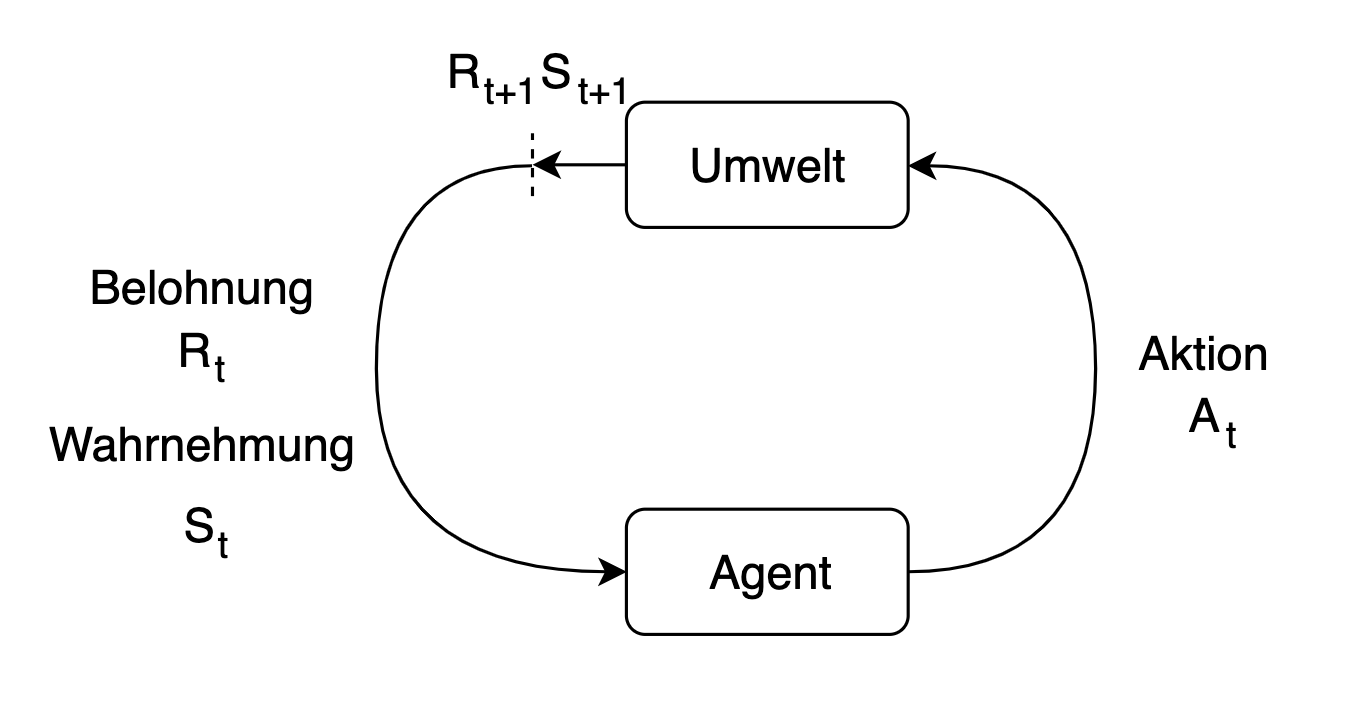
\includegraphics[height=150px]{images/agentUmweltInterface.png}
    \caption{Agent-Umwelt Interface}
\end{figure}


Der Agent interagiert mit dem \textit{MDP} jeweils zu diskreten Zeitpunkten $t = 0, 1, 2, 3, \dots$. \\
Zu jedem Zeitpunkt $t$ beobachtet der Agent den Zustand seiner Umgebung $S_t \in \mathcal{S}$ und wählt aufgrund dessen eine Aktionen $A_t \in \mathcal{A}$. Als Konsequenz seiner Aktion erhält er einen Zeitpunkt später eine Belohnung $R_{t+1} \in \mathcal{R} \subset\mathbb{R} $ und stellt den Folgezustand $S_{t+1}$ fest. 
\par 
In der Literatur findet sich jedoch auch eine abweichende Definition im Bezug auf den Zeitpunkt der Belohnungsvergabe. \cite{watkins1989learning}, \cite{Wiering} und \cite{YuMDP} z.B. binden die Belohnung $R_t$ an das Zustands-Aktions-Paar $(S_t, A_t)$. Die  Definition $R_{t+1}$ bei Aktion $A _{t}$ von \cite{Sutton1998} wird allerdings im Verlauf dieser Arbeit verwendet, da sie besser beschreibt, dass die Belohnung und der Folgezustand gemeinsam berechnet werden und einen Zeitpunkt später, nach Aktion $A_t$, für den Agenten sichtbar sind.
\par 
Das Zusammenspiel zwischen Agenten und MDP erzeugt somit folgende Reihenfolge \cite[~S.48]{Sutton1998}:

\begin{equation}\label{eq:episode}
    S_0, A_0, R_1, S_1, A_1, R_2, S_2, A_2, R_3, \dots
\end{equation}

Wird einfach nur von \textit{MDPs} gesprochen, ist die endliche Variante (\textit{finite MDP}) gemeint, bei dem die Mengen der Zustände, Aktionen und Belohnungen ($\mathcal{S}, \mathcal{A}, \mathcal{R}$) eine endliche Anzahl an Elementen besitzen. In diesem Fall haben die Zufallsvariablen $R_t$ und $S_t$ wohl definierte, diskrete Wahrscheinlichkeitsverteilungen, die nur von dem vorigen Zustand und der vorigen Aktion abhängig sind. Die Wahrscheinlichkeit, dass die bestimmten Werte für diese Variablen $s' \in \mathcal{S}$ und $r \in \mathcal{R}$ eintreten, für einen bestimmten Zeitpunkt $t$ und dem vorigen Zustand $s$ und Aktion $a$, kann somit durch folgende Funktion beschrieben werden \cite[~S.48]{Sutton1998}:

\begin{equation}\label{eq:übergangsfunktion}
p(s',r \mid s,a) \doteq Pr\{S_t=s',R_t=r|S_{t-1}=s,A_{t-1}=a\},
\end{equation}

für alle $s', s \in \mathcal{S}, r \in \mathcal{R}$ und $a \in \mathcal{A}(s)$. Diese Funktion $p$ definiert die sog. Dynamiken (\textit{Dynamics}) eines \textit{MDP}. Sie ist eine gewöhnliche deterministische Funktion mit vier Parametern $p: \mathcal{S} \times \mathcal{R} \times \mathcal{S} \times \mathcal{A} \rightarrow [0,1]$. Das \glqq$\mid$\grqq{} Zeichen kommt ursprünglich aus der Notation für bedingte Wahrscheinlichkeiten, soll hier aber andeuten, dass es sich um eine Wahrscheinlichkeitsverteilung handelt für jeweils alle Kombinationen von $s$ und $a$ \cite[~S.49f]{Sutton1998}:

\begin{equation}\label{eq:wahrscheinlichkeitsverteilung}
\sum_{s' \in \mathcal{S}} \sum_{r \in \mathcal{R}} p(s', r \mid s,a) = 1 \ \forall s \in \mathcal{S}, a \in \mathcal{A}(s)
\end{equation}

Ist das Entscheidungsproblem nicht stochastischer Natur, sondern deterministisch, so ist $p$ immer nur für ein bestimmtes Triplet $(s,a,r)$ für jedes $s' \in \mathcal{S}$ gleich 1, für alle andere jeweils 0. Mit anderen Worten, wird im Zustand $s$ die Aktion $a$ gewählt, führt dies in jedem Fall zu einem bestimmten Folgezustand $s’$. 
\par 

\cite{Sutton1998} erläutern, dass das MDP Framework als extrem flexibel gilt und es demzufolge auf die unterschiedlichsten Probleme angewendet werden kann. Sie führen weiter aus, dass es die nötige Abstraktion für Probleme bietet, bei denen unter Vorgabe eines Ziels mittels Interaktionen gelernt wird. Einzelheiten über das eigentliche Ziel, die Zustände oder die Form des Agenten sind dabei unerheblich. 
Letztendlich kommen die zwei Autoren zu dem Schluss, dass \glqq jedes zielgerichtete Lernen auf drei Signale reduziert werden kann, die zwischen dem Agenten und der Umwelt ausgetauscht werden. Ein Signal repräsentiert die Entscheidung, die der Agent getroffen hat (die Aktion), ein Signal repräsentiert die Basis, auf der er zu dieser Entscheidung gekommen ist (der Zustand) und ein Signal definiert das zu erreichende Ziel (die Belohnung)\grqq{} (S.~50).



	\subsection{Markow-Eigenschaft und Zustandsmodellierung}
	Die Markow-Eigenschaft, obwohl relativ simpel, erhält ein eigenes Kapitel, da sie von fundamentaler Wichtigkeit ist und bei der Modellierung eines Reinforcement Learning Problems eine besondere Rolle spielt. Verbinden lässt sich dies sehr gut mit einem Einblick über die grundsätzliche Modellierung von Zuständen bei einem Reinforcement Learning Problem.

\begin{quote}
    The future is independent of the past given the present
  \end{quote}

Dieser Satz erscheint oft in Büchern und Papern, wenn es um die Markov-Eigenschaft geht, denn er versucht zusammenzufassen, was diese aussagt. Im Zusammenhang von MDPs lässt sich dieser Satz so übersetzen, dass ein Folgezustand nicht abhängig von Aktionen bzw. Zuständen in der Vergangenheit ist, sondern ausschließlich von dem aktuellen Zustand und der aktuell gewählten Aktion.
In der Literatur gibt es unterschiedliche Auffassungen darüber, ob die Markov-Eigenschaft an den MDP direkt geknüpft ist oder an den Zustand, den der Agent zur Abwägung der Entscheidung zur Verfügung hat. Bei der ersten Annahme wird davon ausgegangen, dass der Zustand, der von der Umwelt ausgeliefert wird direkt die Markov-Eigenschaft besitzen muss. (Sutton S.49) hingegen bindet die Eigenschaft an den Zustand und nicht an den Entscheidungsprozess als solches. Ein Zustand ist somit die Menge aller notwendigen Informationen der Vergangenheit, die für die Zukunft relevant sind. Statt den gegebenen Zustand der Umwelt direkt zu übernehmen, werden hier Beobachtungen der Umwelt zu einer internen Repräsentation von Markov-Zuständen verarbeitet.


% \begin{figure}[H]
%     \centering
%     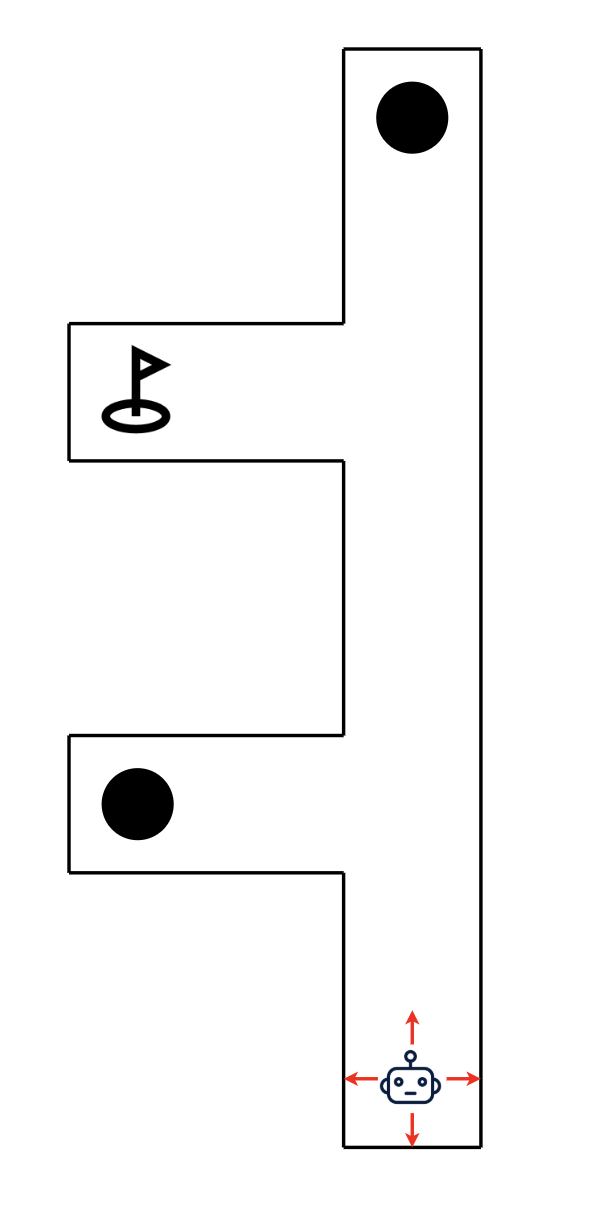
\includegraphics[height=250px]{images/2passagesDefault.png}
%     \caption{ Zwei-Wege Beispiel zu der Markov-Eigenschaft}
% \end{figure}

% \begin{wrapfigure}{L}{0.5\textwidth}
%   \begin{center}
%   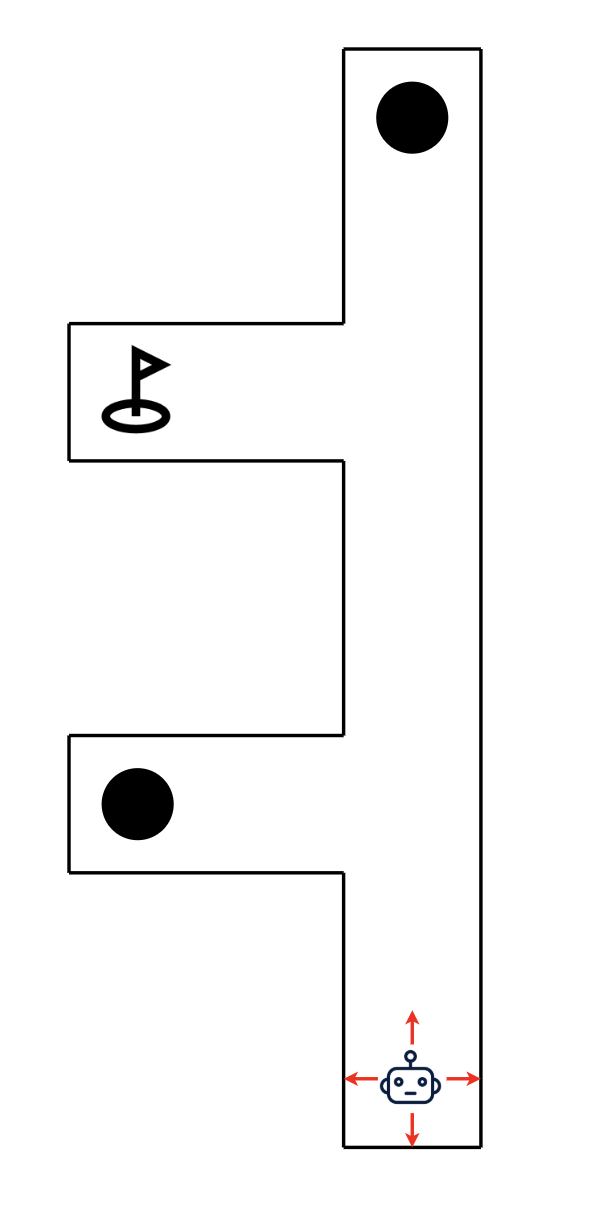
\includegraphics[height=250px]{images/2passagesDefault.png}  \end{center}
%   \caption{Birds}
% \end{wrapfigure}

	\pagebreak

	\subsection{Belohnungen und Zielstrebigkeit}
	Das Besondere an dem Reinforcement Learning ist das Belohnungssignal (\textit{Reward}), welches der Agent nach jeder Aktion erhält. Zu jedem diskreten Zeitpunkt wird dem Agenten eine Belohnung in Form einer einfachen Zahl $R_t \in \mathbb{R}$ zugestellt. Aufgabe eines jeden RL-Algorithmus ist es, die Summe aller gesammelten Belohnungen zu maximieren. Dabei ist entscheidend, dass der Fokus nicht ausschließlich auf die sofortigen Belohnungen gerichtet ist, sondern auf die erwartbare Summe aller Belohnungen über einen langen Zeitraum. Entscheidungen, die in der Gegenwart eine hohe sofortige Belohnungen versprechen sind verführerisch, können sich aber in der Zukunft in Bezug auf den gesamten Prozess als suboptimal herausstellen. 
\par 
Eine Belohnungsfunktion wird in der Regeln von einem Menschen definiert und hat den größten Einfluss darauf, wie der Agent sich verhalten soll. Die Festlegung von Belohnung bei bestimmten Events ist die einzige Möglichkeit, die der Agent hat, zu verstehen, welches Ziel er verfolgen soll. Somit ist die Modellierung der passenden Belohnungsfunktion zur korrekten Abbildung der eigentlichen Aufgabenstellung von gravierender Bedeutung.
\par 
Grundsätzlich gibt es zwei Ansätze, um eine Belohnungsfunktion zu formulieren. Verständlich werden diese durch ein Beispiel, bei dem ein Agent lernen soll, Schach zu spielen. Die erste Möglichkeit besteht darin, dem Agenten ausschließlich eine Belohnung aufgrund des Spielausgangs zu geben. Er erhält +1 wenn er gewinnt, -1 bei einer Niederlage und 0 bei Unentschieden (und jeder Aktion zuvor). Auf den ersten Blick erscheint dieser Ansatz trivial, ist aber die direkte Übersetzung des Ziels in eine Belohnungsfunktion. Die größte erwartbare Summe aller Belohnungen erhält der Agent nur, wenn er lernt, das Spiel zu gewinnen. Größter Nachteil dieser Methode ist allerdings, dass der Agent keinerlei Hilfe oder Richtung beim Erkunden des Spiels erhält. Je größer der Zustands- und Aktionraum ist, desto länger braucht er um überhaupt einmal ein Spiel gewinnen zu können und zu lernen, welche Aktionen vorteilhaft sind und welche nicht.
\par 
Um dem entgegenzuwirken, werden dem Agenten bei der zweiten Möglichkeit feingranularere Belohnungen mitgeteilt, statt diese ausschließlich auf das Endresultat zu reduzieren. Bestimmte Belohnungen zeigen dann, ob der Agent seinem Ziel näher gekommen ist oder eine ungünstige Entscheidung getroffen hat. Zum Beispiel könnte dem Agenten eine hohe Belohnung von +10 gegeben werden, wenn er die gegnerische Dame aus dem Spiel nimmt. Es ist auch denkbar, dass jede Spielfeldkonstellation bewertet wird. Dieser Ansatz benötigt somit spezielles Vorwissen über das Problem und kann sich zugleich sehr negativ auf das Verfolgen des eigentlichen Ziels auswirken. Der Agent könnte zum Beispiel nur lernen in jedem Spiel die Dame des Gegners zu schlagen und dabei trotzdem immer die Partie zu verlieren.
\par 
Die korrekte Modellierung der Belohnungsfunktion hat somit eine besondere Bedeutung. Im Beispiel von Schach sollte nur aufgrund des Spielaussgangs bewertet werden. Durchläuft der Agent allerdings ein Labyrinth und soll er so schnell wie möglich hinausfinden, dann sollte nach jeder Aktion eine negative Belohnung von -1 verteilt werden. Somit wird der Agent gezwungen, auf direktem Wege den Zielzustand zu erreichen.
\par 
Prinzipiell gilt: Das Belohnungssignal dient dazu, dem Agenten mitzuteilen \textit{was} er erreichen soll, nicht \textit{wie} er es erreichen soll\cite[S.~54]{Sutton1998}.

	\subsection{Gewinn und Episoden}
	In Kapitel 2.1 wurde gezeigt, dass die Interaktion eines Agenten mit seiner Umwelt als bestimmte Abfolge beschrieben werden kann \eqref{eq:episode}. In ihr werden letztendlich alle Triples von Zustand, ausgeführter Aktion aufgrund dieses Zustands und anschließende Belohnung chronologisch aufgezeichnet. Ist diese Reihenfolge endlich, so wird sie auch als Episode (\textit{Episode}) bezeichnet. Eine Episode fasst somit alle Informationen zusammen, die ein Agent erlebt, während er von einem beliebigen Startzustand aus anfängt die Umwelt zu erkunden. Das Ende einer Episode wird durch das Erreichen eines beliebigen Zielzustands erreicht. Ist eine Episode zu Ende, dann wird das Szenarie zurückgesetzt und der Agent startet erneut im Startzustand. Episoden sind komplett unabhängig voneinander und erzeugen Trajektorien, die nicht von durch vorrige Episoden beeinflusst werden.
\par
Bisher wurde erwähnt, dass das Ziel eines Agenten sei, die Summe der zu erwartenden Belohnungen zu maximieren. Formal betrachtet, versucht er somit die Sequenz der Belohnung, die er nach dem Zeitpunkt $t$ erhält, den sog. erwarteten Gewinn (\textit{Return}), zu maximieren. Im einfachsten Fall sieht $G_t$ wie folgt aus, wobei $T$ der finale Zeitstempel ist.

\begin{equation}\label{eq:simpleReturn}
    G_t = R_{t+1} + R_{t+2} + R_{t+3} + \dots + R_{T}
\end{equation}

Diese simple Addition von nachfolgenden Belohnungen ist ausreichend und sehr praktikabel bei episodialen Problemszenarien. Jedoch ungeeignet für Probleme, bei denen keine klaren Endzustände definiert sind und daher einen sog. unendlichen Horizont (infinite horizon) besitzen. Folglich ist  $T=\infty$, was wiederum bedeutet, dass der Gewinn ebenfalls unendlich ist. 
\par 
Um episodiale und kontinuierliche Aufgaben im Bezug auf den Gewinn zu vereinheitlichen, wird das Konzept der Diskontierung (\textit{discounting}) verwendet. Dabei gibt der Parameter $\gamma$, $0\leq \gamma \leq 1$, Auskunft darüber, wie die Gewichtung zwischen sofortigen und zukünftigen Belohnungen verteilt ist. Der zukünftige diskontierte Gewinn, der durch die Aktion $A_t$ maximiert werden soll, berechnet sich somit wie folgt:

\begin{equation}\label{eq:discountedReturn}
    G_t = R_{t+1} + \gamma R_{t+2} + \gamma^2 R_{t+3} + \dots  = \sum_{k=0}^\infty{\gamma^k R_{t+k+1}}
\end{equation}
Weiterhin ist zu vermerken, dass Gewinne von aufeinanderfolgenden Zeitpunkten miteinander verbunden sind \cite[S.55]{Sutton1998}.

\begin{equation}\label{eq:successiveReturn}
    \begin{aligned}
    G_t &= R_{t+1} + \gamma R_{t+2} + \gamma^2 R_{t+3} + \gamma^3 R_{t+4} + \dots \\
    &= R_{t+1} + \gamma (R_{t+2} + \gamma R_{t+3} + \gamma^2 R_{t+4} + \dots)  \\
   & = R_{t+1} + \gamma G_{t+1}
    \end{aligned}
\end{equation}
Ist $\gamma = 0$, dann wählt der Agent seine Aktionen ausschließlich aufgrund der sofortigen Belohnung. Je näher $\gamma$ an 1 ist, desto "weitsichtiger" wird der Agent, da der Gewinn für den Zeitpunkt $t$ sich zusätzlich aus zukünftigen Belohnungen zusammensetzt. Bei Problemen, die sich in Episoden unterteilen lassen, ist es üblich, dass $\gamma = 1$ ist, sodass der Agent seine Entscheidungen immer aufgrund jeglicher Konsequenzen in der Zukunft bzw. bis zum Ende der jeweiligen Episode trifft. Um zu erreichen, dass die unendliche Summe in \eqref{eq:discountedReturn} bei kontinuierlichen Aufgaben einen endlichen Wert annimmt, muss $\gamma < 1$ \cite[S.55]{Sutton1998}. 
\par 
Probleme mit unendlichen Horizont können durch die Vergabe einer künstlichen Schranke zu einer episodialen Aufgabe umformuliert werden. Denkbar z.B. durch die Festlegung der maximalen Anzahl an Aktionen oder besuchten Zustände. 
\par 
Die Algorithmen der Monte-Carlo-Methoden, die in Kapitel X vorgestellt werden, können ausschließlich auf Basis von Episoden lernen. Jedoch existieren auch Methoden, wie das Temporal-Difference-Learning (Kapitel X), die neben dem episodialen Lernen, zusätzlich in der Lage sind, mit kontinuierlichen Aufgaben zurechtzukommen. 

	\subsection{Strategie und Nutzenfunktion}
	Fast alle Lernalgorithmen des Reinforcement Learning versuchen eine sog. Nutzenfunktion (\textit{Value Function}) zu schätzen. Diese Funktion sagt aus, \glqq wie gut\grqq{} es ist, dass sich der Agent in einem bestimmten Zustand befindet oder eine bestimmte Aktion in einem Zustand ausführt. Dabei bezieht sich das \glqq wie gut\grqq{} darauf,
welche Belohnungen in der Zukunft erwartbar sind, dementsprechend wie groß der erwartete Gewinn ist. Zukünftige Belohnungen sind natürlicherweise abhängig davon, wie sich der Agent verhalten oder vielmehr welche Entscheidungen er in der Zukunft treffen wird. Nutzenfunktion sind deshalb immer in Bezug auf eine bestimmte Strategie definiert \cite[S.~58]{Sutton1998}.
\par 
Eine Strategie (\textit{Policy}) kann als Abbildung verstanden werden, die jedem Zustand eine diskrete Wahrscheinlichkeitsverteilung über Aktionen zuordnet. Folgt der Agent einer Strategie $\pi$ zum Zeitpunkt $t$, dann gibt $\pi(a\mid s)$ an, mit welcher Wahrscheinlichkeit $A_t = a$ ausgeführt wird, wenn $S_t = s$ \cite[S.~58]{Sutton1998}. Neben solchen stochastischen Strategien, existieren auch simplere, deterministische Strategien, die jedem Zustand nur genau eine Aktion zuordnen, $\pi (s) = a$ \cite[]{Brunskill}.
\par
Wie anfangs erwähnt, gibt es zwei Varianten der Nutzenfunktion. Die erste sagt aus, wie groß der Erwartungswert des Gewinns für den Zustand $s$ ist, wenn in diesem gestartet und anschließend aufgrund der Strategie $\pi$ gehandelt wird. Dieser \textit{Zustands-Nutzen} kann für alle $s \in \mathcal{S}$ folgendermaßen definiert werden \cite[S.~58]{Sutton1998}:
\begin{equation}\label{eq:valueFunction}
    v_\pi(s) = \EX_\pi[G_t \mid S_t = s] = \EX_\pi \left[\sum_{k=0}^\infty{\gamma^k R_{t+k+1} \mid S_t = s} \right]
\end{equation}

Die zweite Variante gibt Auskunft darüber, wie groß der Nutzen ist, wenn im Zustand $s$ gestartet, daraufhin die Aktion $a$ ausgeführt und anschließend der Strategie $\pi$ gefolgt wird. $q_\pi$ wird auch als \textit{Aktions-Nutzenfunktion} für die Strategie $\pi$ bezeichnet und wird formal ausgedrückt durch \cite[S.~58]{Sutton1998}:
\begin{equation}\label{eq:actionValueFunction}
    q_\pi(s,a) = \EX_\pi[G_t \mid S_t = s, A_t = a] = \EX_\pi\left[\sum_{k=0}^\infty{\gamma^k R_{t+k+1} \mid S_t = s, A_t = a}\right]
\end{equation}

//TODO der Erwartungswert auf ?
//TODO funktionsapproximation hier? 

	\subsection{Optimalität}
	Ein Reinforcement Learning Problem zu lösen bedeutet, eine Strategie zu finden, die den größten Gewinn bringt. Dabei lassen sich Strategien vergleichen, insofern, dass eine Strategie besser als eine andere ist, wenn der erwartete Gewinn für alle Zustände größer oder gleich ist \cite[S.~62f]{Sutton1998}. Mit anderen Worten, $\pi \geq \pi'$ gilt, wenn $v_\pi(s) \geq v_{\pi'}(s)$ für alle $s \in \mathcal{S}$. Es existiert mindestens eine Strategie, die besser oder gleich gegenüber allen anderen Strategien ist. Diese ist die optimale Strategie $\pi_*$. \newpage
Optimale Strategien teilen dieselbe (optimale) Zustands-Nutzenfunktion $v_*$ und (optimale) Aktions-Zustands-Nutzenfunktion $q_*$ \cite[S.~62f]{Sutton1998}:

\begin{equation}\label{eq:optimaleValueFunction}
    v_*(s) = \max_\pi v_\pi(s)
\end{equation}
\begin{equation}\label{eq:optimaleActionValueFunction}
    q_*(s,a) = \max_\pi q_\pi(s,a)
\end{equation}

Nutzenfunktionen sind, wie im vorigen Kapitel erläutert, immer abhängig von einer bestimmten Strategie, da diese die gesammelte Erfahrung und somit gleichermaßen die erwarteten, geschätzten Gewinne beeinflusst. Die optimale Nutzenfunktion kann jedoch auch ohne Referenz auf eine konkrete Strategie beschrieben werden, da der Gewinn eines Zustands unter einer optimalen Strategie gleich dem erwarteten Gewinn für die beste Aktion in diesem Zustand ist. $v_*(s)$ referenziert somit $v_*(s')$, den besten Folgezustand, wodurch eine rekursive Beziehung zustande kommt. Eine optimale Nutzenfunktion $v_*$ kann formal folgendermaßen beschrieben werden \cite[S.~63]{Sutton1998}:

\begin{equation}\label{eq:bellmanValue}
    \begin{aligned}
        v_*(s) &= \max_a \EX_{\pi_*}[G_t | S_t = s, A_t = a] \\
        &= \max_a \EX{\pi_*}[ R_{t+1} + \gamma G_{t+1} | S_t = s, A_t = a] \\
        &= \max_a \EX[ R_{t+1} + \gamma v_*(S_{t+1}) | S_t = s, A_t = a] \\
        &= \max_a \sum_{s',r}p(s', r | s,a)[r+ \gamma v_*(s')]
    \end{aligned}
\end{equation}

Diese Gleichung ist die sog. \textit{Bellman Optimality Equation} und lässt sich auch als Gleichungssystem interpretieren, welches eine Gleichung pro Zustand besitzt. Für ein Problem mit $n$ Zuständen ergeben sich somit $n$ Gleichung mit $n$ Unbekannten \cite[S.~63]{Sutton1998}. Eine Berechnung der optimalen Nutzenfunktion ist folglich in der Theorie möglich, jedoch muss die Übergangsfunktion $p$ bekannt sein. Ist $p$ gegeben, wird von einem perfekten Modell gesprochen, eine Voraussetzung, die nicht immer erfüllt ist.
\par 
Selbst wenn die Dynamiken der Umwelt bekannt sind, kann die benötigte Rechenzeit zur Lösung jedoch utopische Ausmaße annehmen. Bei einem Spiel wie \glqq Backgammon\grqq{} sind die Regeln klar definiert, ein perfektes Modell ist demzufolge vorhanden, aber es existieren $10^{23}$ Zustände, was die mathematische Berechnung von $v_*$ mit der \textit{Bellman Optimality Equation} praktisch unmöglich macht \cite[S.~66]{Sutton1998}. Dennoch stellt sie ein wichtiges Fundament für das Reinforcement Learning dar, da die meisten Reinforcement Learning Algorithmen als annäherungsweises Lösungsverfahren verstanden werden können \cite[S.~66]{Sutton1998}. 
\newpage
Methoden des Reinforcement Learnings, die die Umwelt als Blackbox betrachten, werden auch als \textit{model-free} beschrieben. Sie benötigen keinen Zugriff auf die Übergangsfunktion $p$, denn es wird ausschließlich aufgrund der erhaltenen Belohnungen und Beobachtungen gelernt. Hierbei bezieht sich der Lernprozess darauf, wie nah die geschätzte Nutzenfunktion der aktuellen Strategie $\pi$ an $v_*$ bzw. $q_*$ ist.
\par 
Die optimale Strategie lässt sich leicht ermitteln, wenn eine optimale Nutzenfunktion gegeben ist. Ist zum Beispiel $v_*$ vorhanden und befindet sich der Agent in Zustand $s$, dann muss er eine Aktion vorausschauen, um den Folgezustand $s'$ zu finden, der den maximalen Nutzen hat. Dieses Voraussehen benötigt jedoch ein perfektes Modell der Umgebung, um die Übergänge für jede Aktion zu berechnen. Das ist der ausschlaggebende Grund, warum bei \textit{model-free} Methoden $q_*$ berechnet wird. Denn dieser Nutzen umfasst implizit den Nutzen der Folgezustände für jede Aktion. Infolgedessen muss der Agent im Zustand $s$ nur evaluieren, welche Aktion $a$ und somit welches Zustands-Aktions-Paar den größten Nutzen hat und wählt genau jene Aktion.
\par 

\par 

\bibliographystyle{apacite}
\bibliography{quellen}
\pagebreak

Bellman Optimality Equation:
\begin{equation}\label{eq:bellman}
    \begin{aligned}
    q_*(s,a) &= \EX [R_{t+1} + \gamma \max_{a'}q_*(S_{t+1}, a') \mid S_t = s, A_t = a] \\
    &= \sum_{s',r}p(s', r\mid s, a)[r + \gamma \max_{a'}q_*(s', a')]
    \end{aligned}
\end{equation}
\end{document}
